%------------------
% General Settings
%------------------
\def \docTitle      {User Manual}
\def \docSubTitle   {SMC2242/SMC4242}
\def \productNumber {SMCx242}
\def \productName   {Stepper Motor Controller}
\def \docAuthor     {LK-Instruments}
\def \docSubject    {\docAuthor \docTitle \docSubTitle}
\def \docKeywords   {LK-Instruments, Stepper Motor Controller, SMC2242, SMC4242}

%\documentclass[a4paper, final, 12pt, twoside]{scrartcl}
\documentclass[a4paper, final, 12pt, oneside]{refart}

%----------
% Packages
%----------
\usepackage{etex}
\reserveinserts{30}
\usepackage[utf8]{inputenc}
%\usepackage[latin1]{inputenc} % erlaubt Umlaute in der tex-Datei

\usepackage{slantsc}
\usepackage[urw-garamond]{mathdesign}
\usepackage{garamondx}
\usepackage[T1]{fontenc}

\usepackage[english]{babel}              % For the hyphenations in different languages
\usepackage[intlimits]{amsmath}          % math symbols
\usepackage{braket}                      % Dirac braket notation
\usepackage{graphicx}                    % include pictures
\usepackage{color}
%\usepackage[shell]{gnuplottex}           % gnuplot in latex
\usepackage{pstricks}                    % post script tricks
\usepackage{listings}                    % enter programming code
\usepackage{fancyhdr}                    % make quite nice header/footer
%\usepackage[version=3]{mhchem}           % chemistry stuff
\usepackage{relsize}
\usepackage{afterpage}
\usepackage{gensymb}
\usepackage{textcomp}
\usepackage{listings}					 % erlaubt Quellcode mit Zeilenumbruechen
\usepackage{makeidx}                     % create index
  \makeindex
\usepackage{lcd}						 % Character LCD
%\usepackage[paperheight=210mm,paperwidth=210mm,margin=20mm,heightrounded]{geometry}
\usepackage{multirow}
\usepackage{booktabs}
\usepackage{colortbl}
\usepackage{tabularx}


\usepackage{pgfplots}
\usepackage{tikz}                        % beautiful plots
\pgfplotsset{compat = newest}
\usepackage{units}                       % easy to use number-unit-package
\usepackage[section]{placeins}           % Float barrier for sections.

\usepackage{float}                       % lädt das Paket zum erzwingen der Grafikposition

\usetikzlibrary{shapes.geometric, arrows}	% Flow chart

\newfont{\ce}{cerm}                      
\def\CE#1{{\font\ce=#1\ce CE}}


%----------------
% PDF properties
%----------------
\usepackage[
  pdftitle={\docAuthor~\docSubTitle~\docTitle}
 ,pdfsubject={\docSubject}
 ,pdfauthor={\docAuthor}
 ,pdfkeywords={\docKeywords}
 ,pdfcreator={\docAuthor}
 ,pdfstartview=Fit                       % startseite ganz anzeigen
 ,pdfborder={0 0 0}                      % links ohne umrandungen
 ,pdfdisplaydoctitle=true                % pdftitle statt dateinamen anzeigen
 ,pdfcenterwindow=true                   % position pdf in center of the screen
 ,setpagesize=true
]{hyperref}

%-------------------
% Header und Footer
%-------------------
\pagestyle{fancy}
\fancyhf{}        % clear all header/footer
\renewcommand{\headrulewidth}{0pt}
\renewcommand{\sectionmark}[1]{\markboth{#1}{}}
\renewcommand{\subsectionmark}[1]{\markright{#1}}
\fancyhead[LE,RO]{\textbf{\thepage}}
\fancyhead[CE]{\footnotesize{\textit{\nouppercase{\rightmark}}}}
\fancyhead[CO]{\footnotesize{\scshape{\nouppercase{\leftmark}}}}

% number equations with sections before equation-index
\numberwithin{equation}{section}
\numberwithin{table}{section}
\numberwithin{figure}{section}

%---------------------
% My code definitions
%---------------------

\newtheorem{envdefinition}{Definition}[section]
\newtheorem{envsatz}{Satz}

% special numbers and letters
\renewcommand{\i}{\mathrm{i}}                  % complex i
\newcommand{\e}{\mathrm{e}}                    % Eulers number
\renewcommand{\phi}{\varphi}                   % nicer phi
\renewcommand{\epsilon}{\varepsilon}           % nicer epsilon
\renewcommand{\theta}{\vartheta}               % nicer theta
\renewcommand{\rho}{\varrho}                   % nicer rho
%\newcommand{\degree}{^{\circ}}                 % degree-circle

% vectors and matrices
\renewcommand{\vec}[1]{\boldsymbol{#1}}
\newcommand{\Vek}[3]{\left(\begin{array}{c}#1\\#2 
\ifthenelse{\equal{#3}{}}{}{\\#3}\end{array}\right)}

% integral and derivative stuff:
\renewcommand{\d}[1]{\;\mathrm{d}#1}           % integeration d
% total derivative
\newcommand{\td}[1]{\frac{\mathrm{d}}{\mathrm{d}#1}\,}
\newcommand{\pd}[1]{\partial_{#1}\,}             % partial derivative

% Braket notation
\renewcommand{\bra}{\Bra}
\renewcommand{\ket}{\Ket}
\renewcommand{\braket}{\Braket}
\renewcommand{\set}{\Set}

% plus-minus with braces
\newcommand{\PM}{\ensuremath{\substack{+\\[-0.25em]-}\,}}
\renewcommand{\pm}{\PM}
\newcommand{\pmp}{\ensuremath{\substack{\mathsmaller{(}+\mathsmaller{)}\\[-0.25em]-}\,}}
\newcommand{\pmm}{\ensuremath{\substack{+\\[-0.25em]\mathsmaller{(}-\mathsmaller{)}}\,}}

%---------------------
% LCD
%---------------------

\definecolor{lightgrey}{rgb}{0.9,0.9,0.9}
\definecolor{darkgrey}{rgb}{0.2,0.2,0.2}
\definecolor{black}{rgb}{0,0,0}
\LCDcolors{black}{lightgrey}


%---------------------
% Index
%---------------------


%----------------------------------------------------------
% let the party start
%----------------------------------------------------------
\begin{document}


\pagecolor{black}
.
\vspace{4cm}
\begin{center}
  
\includegraphics[width=0.6\textwidth]{../general/logo_white.pdf}
\end{center}

\vspace*{2cm}
\begin{center}
  {\color{white} \Huge\textbf{\textsf{\docTitle}}}
\end{center}

\vspace*{1cm}
\begin{center}
  {\color{white} \Huge\textbf{\textsf{\productName}}}
\end{center}

%\vspace*{0.5cm}
\begin{center}
  {\color{white} \Huge\textbf{\textsf{\docSubTitle}}}
\end{center}

\afterpage{\nopagecolor}
\newpage


\thispagestyle{empty}
\section*{Notices}
\textcopyright~\docAuthor~2016.
No part of this manual may be reproduced in any form or by any means
(including electronic storage and retrieval or translation into a
foreign language) without prior agreement and written consent from \docAuthor.

\subsection*{Edition}
\today

\subsection*{Warranty}
The material contained in this document is provided \glqq as is\grqq, and is subject to
being changed, without notice, in future editions. Further, to the maximum extent
permitted by applicable law, \docAuthor~disclaims all warranties, either express or
implied, with regard to this manual and any information contained herein,
including but not limited to the implied warranties of merchantability and fitness
for a particular purpose.

\docAuthor~ shall not be liable for errors or for incidental
or consequential damages in connection with the furnishing, use, or performance of
this document or of any information contained herein. Should \docAuthor~and
the user have a separate written agreement with warranty terms covering the material
in this document that conflict with these terms, the warranty terms in the
separate agreement shall control.

\subsection*{Technology Licenses}
The hardware and/or software described in this document are furnished under a
license and may be used or copied only in accordance with the terms of such license.

%\subsection*{Restricted Rights Legend}
%If software is for use in the performance of a U.S. Government prime contract or
%subcontract, Software is delivered and licensed as “Commercial computer software”
%as defined in DFAR 252.227-7014 (June 1995), or as a “commercial item” as defined
%in FAR 2.101(a) or as “Restricted computer software” as defined in FAR 52.227-19
%(June 1987) or any equivalent agency regulation or contract clause. Use,
%duplication or disclosure of Software is subject to BitifEye’s standard commercial
%license terms, and non-DOD Departments and Agencies of the U.S. Government will
%receive no greater than Restricted Rights as defined in FAR 52.227-19(c)(1-2)
%(June 1987). U.S. Government users will receive no greater than Limited Rights as
%defined in FAR 52.227-14 (June 1987) or DFAR 252.227-7015 (b)(2) (November 1995),
%as applicable in any technical data.

%\subsection*{Safety Notices}


%\subsection*{Product Labels}
%\begin{itemize}
%  \item[\CE{cerm scaled \magstep5}] This electronic product is in compliance
%                                    with the EMC and Safety regulations of
%                                    the European Community.
%\end{itemize}



\newpage

\section{Technical Assistance}
If you need product assistance or if you have suggestions, contact \docAuthor.
You will find the contact information on the \docAuthor~homepage at
\begin{center}
  \url{http://www.lk-instruments.com}
\end{center}
Representatives of \docAuthor~are available during standard German business hours.
Before you contact \docAuthor, please note the actions you took before you experienced
the problem. Then describe those actions and the problem to the technical support
engineer.

\subsection{Found a mistake?}
We encourage comments about this publication. Please report any mistakes
to \docAuthor:
\begin{center}
  \href{mailto:support@lk-instruments.com}{\nolinkurl{support@lk-instruments.com}}
\end{center}






\newpage
\clearpage

\pagenumbering{roman}   % small roman page numbering

\tableofcontents
\newpage

\listoffigures
\listoftables

\newpage
\clearpage
\pagenumbering{arabic}  % now arabic page numbering
                        % for the rest of the document
\newpage


Thank you for purchasing the \productNumber ~\productName. This user
manual will explain you how to operate the \productName. Please take
some time to read it carefully before operating the device. Keep the
instructions in a safe place for future reference.

\section{Introduction}
The \productNumber ~\productName ~is a universal controller for  bipolar stepper motors. It can be used to drive two (SMC2242) or four (SMC4242) stepper motors.
% There are three different firmware version available SMCx242-R for rotary axis, SMCx242-L for linear motion and SMCx242-U which features both options.
It is designed to work perfectly together with  our assortment of stepper motor driven stages, but it might be also used to drive 3\textsuperscript{rd} party motors or stages.

\subsection{Package contents}
Please check that the package contains all the following items:
\begin{itemize}
\item \productNumber ~\productName
%\item Power supply
\item USB cable
\item User Manual
\end{itemize}

\subsection{Installing the device}
The \productName ~is designed for the inside use. Therefore it should not be used outside and kept away from water and moisture. Do not operate the unit near any heat sources or in direct sun light. When installing the device ensure to put it on a flat and leveled surface. Also ensure that there is adequate space around the device for ventilation.\\
After moving the unit to a different location, condensation inside the unit may occur. In this case please wait for some hours before you connect the \productName ~to the power supply.\\
Connect the device only to power sources that meet the specifications written on its rear panel.

\begin{figure}[h]
  \centering
  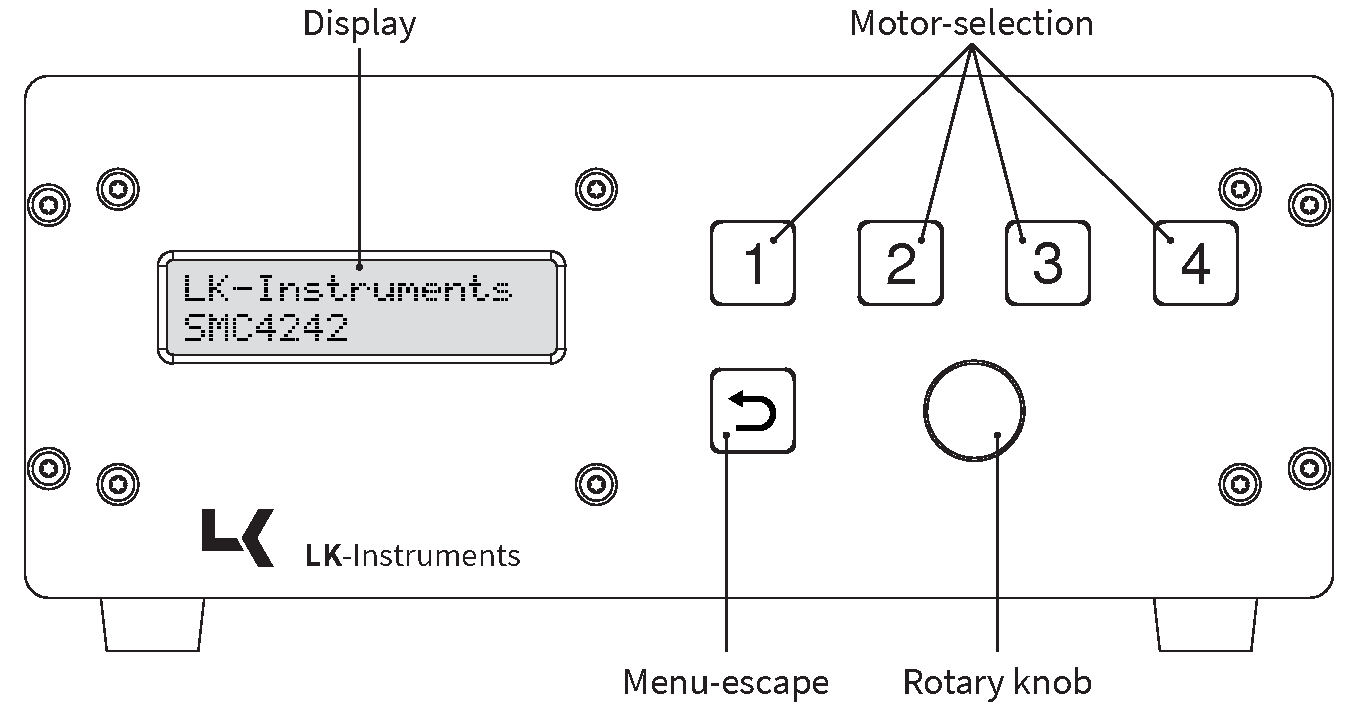
\includegraphics[angle=0,origin=c,width=1\textwidth]{./grafiken/MG22131_front_text_2.pdf}
  \caption[Front view of the \productNumber ~\productName.]{Front view of
  the \productNumber ~    \productName.}
  \label{frontpanel}
\end{figure}

\begin{figure}[h]
  \centering
  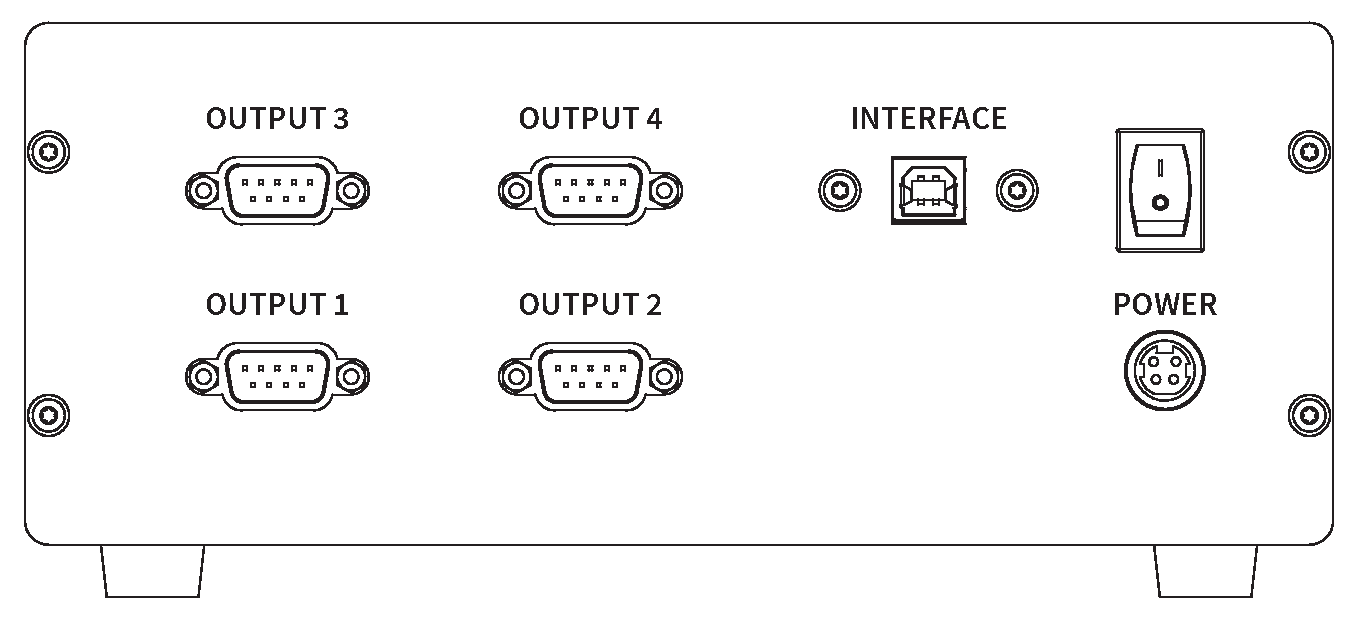
\includegraphics[angle=0,origin=c,width=1\textwidth]{./grafiken/MG22131_back_text.pdf}
  \caption[Rear view of the \productNumber ~\productName.]{Rear view of
  the \productNumber ~    \productName.}
  \label{frontpanel}
\end{figure}



%\newpage
\clearpage
%\section{Basic setup}


\newpage
%\clearpage
\section{General Operation}
The \productNumber ~\productName ~features two operation modes. It can be
either operated using the manual user interface or remote controlled by a
computer. In this section the manual operation of the device is explained.

After turning on the \productName ~it comes up with its start screen.
Turning the rotary encoder serves to scroll through the menus (see
figure~\ref{main_menu}). Pressing the rotary encoder enters the selected
menu. Pressing the menu-escape-button leaves the menu again.

\subsection{Display structure}
In almost every menu four values are displayed. Depending on the previously
selected menu the values correspond to different quantities. Where
\begin{itemize}
  \item the upper left value accompanies to Motor 1
  \item the upper right value accompanies to Motor 2
  \item the lower left value accompanies to Motor 3
  \item the lower right value accompanies to Motor 4
\end{itemize}

\subsection{Motor selection}
To select a motor there are four buttons. Motor selection can solely be
done in an entered menu. To select a motor, press the respective motor-selection
button. A selected motor is signed with an arrow on the display. Pressing the
selection-button again deselects the motor. Once a motor is selected its
appropriate value can be changed by turning the rotary encoder. By leaving
a menu without motor deselection the selected motor(s) stay selected in any
other menu.

\tikzstyle{menu_style} = [rectangle, rounded corners, minimum width=3cm, minimum height=1cm,text centered, draw=black]
\tikzstyle{arrow} = [thick,<->,>=latex]
\def \textWidth {7cm}

\begin{figure}[H]
\begin{tikzpicture}[node distance=2cm]
\node (start) [menu_style] {
\begin{minipage}[h]{5cm}
\LCD{2}{16}|Motor Driver|
|SMC4242|
\end{minipage}
 \hfill
\begin{minipage}[h]{\textWidth}
Start screen\\
Display firmware version.
\end{minipage}
};

\node (motor_pos) [menu_style, below of=start] {
\begin{minipage}[h]{5cm}
\LCD{2}{16}|Change motor|
|position|
\end{minipage}
 \hfill
\begin{minipage}[h]{\textWidth}
%Change motor position:\\
Position is displayed and can be changed.
\end{minipage}
};

\node (step_multiplier) [menu_style, below of=motor_pos] {
\begin{minipage}[h]{5cm}
\LCD{2}{16}|Set step|
|multiplier|
\end{minipage}
 \hfill
\begin{minipage}[h]{\textWidth}
%Set step multiplier\\
Edit multiplier for rotary encoder.
\end{minipage}
};

\node (step_unit) [menu_style, below of=step_multiplier] {
\begin{minipage}[h]{5cm}
\LCD{2}{16}|Change step|
|unit|
\end{minipage}
 \hfill
\begin{minipage}[h]{\textWidth}
%Menu: Change step unit\\
Define the displayed unit.
\end{minipage}
};

\node (optical_zero) [menu_style, below of=step_unit] {
\begin{minipage}[h]{5cm}
\LCD{2}{16}|Define optical|
|zero position|
\end{minipage}
 \hfill
\begin{minipage}[h]{\textWidth}
%Menu: Define optical zero position\\
Edit the zero offset.
\end{minipage}
};

\node (internal_prog) [menu_style, below of=optical_zero] {
\begin{minipage}[h]{5cm}
\LCD{2}{16}|Run internal|
|program|
\end{minipage}
 \hfill
\begin{minipage}[h]{\textWidth}
%Menu: Run internal program\\
Step through the program list.
\end{minipage}
};

\node (const_speed) [menu_style, below of=internal_prog] {
\begin{minipage}[h]{5cm}
\LCD{2}{16}|Set constant|
|angular speed|
\end{minipage}
 \hfill
\begin{minipage}[h]{\textWidth}
%Menu: Set constant angular speed\\
Start/Stop continuous movement.
\end{minipage}
};

\node (step_wait_time) [menu_style, below of=const_speed] {
\begin{minipage}[h]{5cm}
\LCD{2}{16}|Change step|
|wait time|
\end{minipage}
 \hfill
\begin{minipage}[h]{\textWidth}
%Menu: Change step wait time\\
Edit time between steps.
\end{minipage}
};

\node (substep) [menu_style, below of=step_wait_time] {
\begin{minipage}[h]{5cm}
\LCD{2}{16}|Change motor|
|substep|
\end{minipage}
 \hfill
\begin{minipage}[h]{\textWidth}
%Menu: Change motor substep\\
Edit number of substeps.
\end{minipage}
};

%----------------------------------------------------------------------
% zusaetzliche Menues hier einfuegen!
%----------------------------------------------------------------------

\node (save) [menu_style, below of=substep] {
\begin{minipage}[h]{5cm}
\LCD{2}{16}|Save all current|
|configurations|
\end{minipage}
 \hfill
\begin{minipage}[h]{\textWidth}
%Menu: Save all current configurations\\
Save configurations to EEPROM.
\end{minipage}
};

\node (load) [menu_style, below of=save] {
\begin{minipage}[h]{5cm}
\LCD{2}{16}|Load last|
|configuration|
\end{minipage}
 \hfill
\begin{minipage}[h]{\textWidth}
%Menu: Load last configuration\\
Load configuration from EEPROM.
\end{minipage}
};

\node (zero_cal) [menu_style, below of=load] {
\begin{minipage}[h]{5cm}
\LCD{2}{16}|Run zero|
|calibration|
\end{minipage}
 \hfill
\begin{minipage}[h]{\textWidth}
%Menu: Run zero calibration\\
Find mechanical zero position.
\end{minipage}
};

\draw [arrow] (start) -- (motor_pos);
\draw [arrow] (motor_pos) -- (step_multiplier);
\draw [arrow] (step_multiplier) -- (step_unit);
\draw [arrow] (step_unit) -- (optical_zero);
\draw [arrow] (optical_zero) -- (internal_prog);
\draw [arrow] (internal_prog) -- (const_speed);
\draw [arrow] (const_speed) -- (step_wait_time);
\draw [arrow] (step_wait_time) -- (substep);
%------------------------------------------
\draw [arrow] (substep) -- (save);
\draw [arrow] (save) -- (load);
\draw [arrow] (load) -- (zero_cal);
\draw [arrow] (zero_cal.east) -- +(1,0) |- (start.east);
\end{tikzpicture}
\caption[Overview of the available menus.]{Overview of the available menus. By turning
the rotary button one can navigate through the menus as indicated by the arrows.}
\label{main_menu}
\end{figure}

\FloatBarrier



\subsection{Start screen}
By pressing the rotary button while the start screen is active the
firmware version will be displayed.
\begin{center}
  \LCD{2}{16}||
             |v1.3|
\end{center}
Firmware updates are available at \url{http://www.lk-instruments.com} on
the corresponding product website.

\subsection{Motor position}
\label{menu_motor_pos}
\index{change!position}
This menu displays the current motor positions. The position of any motor can be
changed by the operator separately. The default display unit is degree, which
can be changed to the users preferred unit, see \ref{chp:change_step_unit}. The
position of a selected motor can be changed by turning the rotary
button. Default steps for the available units are:
\begin{itemize}
\item $1\degree$ if unit is degree
\item $\frac{\pi}{8}$ if unit is radian
\item 1 step if unit is steps
\end{itemize}
\begin{center}
  \LCD{2}{16}|{rarrow}0.0{pi}   {rarrow}0.0|
             |{rarrow}0st    {rarrow}0.0|
\end{center}


\paragraph{Fast moving mode}
\index{Fast moving mode}
When pressing the rotary button inside the change-motor-position-menu one
enters the fast moving mode. Pressing the rotary button again disables the
fast moving mode. The fast moving mode is indicated by another marking arrow
for the corresponding motor. The fast moving mode will only be enabled or
disabled for selected motors.
Default steps in this mode are:
\begin{itemize}
  \item $10\degree$ if unit is degree
  \item $\frac{\pi}{8}$ if unit is radian
  \item 100 steps if unit is steps
\end{itemize}
The snapped display shows the different indicating arrows. Here, motor 1
and motor 3 are in fast moving mode, motor 2 and 4 are in normal moving mode.
\begin{center}
  \LCD{2}{16}|>17.4  {rarrow}0.0|
             |>0.0   {rarrow}0.0|
\end{center}


\subsection{Step multiplier}
\index{step multiplier}
Step multipliers give the possibility to let the motors move in different
step widths by turning the rotary button one click. It is also possible
to turn the motors in different directions by applying a negative step
multiplier to a motor.

A step multiplier can only be applied if the step unit is degree or radians.
The factory default value for all motors is 1.0.

In this menu one can adjust a step multiplier. The step multiplier is
applied if the step unit is degree or radian. The standard value is 1.0.
If the step multiplier differs from 1.0 the corresponding motor will
rotate more or less steps with each rotation of the rotary encoder.\\
For example: if the step multiplier for motor 0 is 1.0 and the step
multiplier for motor 2 is 4.0, motor 2 will move four times more steps
than motor 0 when changing the motors positions. Negative values are
allowed as well. This will result in counter direction movements.
\begin{center}
  \LCD{2}{16}|{rarrow}1.0x   {rarrow}-0.5x|
             |{rarrow}2.0x    1.0x|
\end{center}

\subsection{Step unit}
\label{chp:change_step_unit}
\index{change!unit}
In this menu one can choose the unit of the displayed position. There
are three possible choices for each motor:
\begin{itemize}
\item degree
\item radian
\item step
\end{itemize}
\begin{center}
  \LCD{2}{16}|{rarrow}radian {rarrow}degree|
             |{rarrow}step    degree|
\end{center}


\subsection{Optical zero position}
\index{optical zero position}
In this menu one can define the optical zero position. This is
necessary due to a mostly unknown placement of the optical element
mounted to the motor. Here one can once adjust the desired optical
zero position manually. The optical zero position is always
defined in steps. In this menu there is also a fast mode available
(please refer to \ref{menu_motor_pos} for details about the fast mode).
After adjustment it is recommended to save this configuration
(see \ref{menu_save}).
When performing a zero calibration, as explained in \ref{menu_zero_cal},
the zero position will be the defined optical zero position.
\begin{center}
  \LCD{2}{16}|{rarrow}122st   0st|
             | 0st     0st|
\end{center}


\subsection{Internal programs}
\index{internal programs}
This menu allows the user to step through the internal program list
with the rotary button.
This function is only available if a program has previously been
defined (see \ref{section_instruction_set}).
Internal programs are also saved to the device when the current
configuration is saved, see \ref{menu_save}.
\begin{center}
  \LCD{2}{16}|Program running|
             |Step 0|
\end{center}


\subsection{Constant angular speed}
Here the motors can be set into an infinite moving state in clockwise
(CW) or counter clockwise (CCW) direction. To get the motors moving
with different velocities one needs to change the wait times between
two steps (see \ref{menu_step_wait_time}).
STOP means that the motor is not moving. Constant angular speed for a
certain motor can not be activated if a forbidden zone is configured to
this motor (see \ref{chp:forbidden_zone}).
\begin{center}
  \LCD{2}{16}|{rarrow}CW     {rarrow}CCW|
             | STOP    STOP|
\end{center}


\subsection{Step wait time}
\label{menu_step_wait_time}
\index{change!step wait time}
Here the wait time between two steps can be changed. This results in
faster or slower motor movements. The default value is 3 milliseconds.
We do not recommend to use shorter wait times as 3 milliseconds.
\begin{center}
  \LCD{2}{16}|{rarrow}3 ms   {rarrow}5 ms|
             |{rarrow}18 ms   3 ms|
\end{center}


\subsection{Motor substeps}
\index{change!substeps}
\index{change!microstepping}
In this menu one can change the motor substeps. Possible values are 1,
2, 4, 8, 16 or 32.
\begin{center}
  \LCD{2}{16}|{rarrow}1      {rarrow}2|
             | 4      {rarrow}8|
\end{center}
This adjustments result in a finer angular resolution. Values above
16 are not recommended.


\paragraph{A note on microstepping.}
\index{microstepping}
When increasing the the number of microsteps per full step the incremental
torque per microstep decreases heavily. The expression for calculating
the incremental tourque $\tau_{\text{inc}}$ is
\begin{equation*}
  \tau_{\text{inc}} = \tau_{\text{H}} \cdot \sin \left( \frac{90}{\mu} \right),
\end{equation*}
where $\tau_{\text{H}}$ is the holding torque per full step (without
microstepping) and $\mu$ is the number of microsteps per full step.\\
The incremental torque $\tau_{\text{N}}$ for $N$ microsteps is
\begin{equation*}
  \tau_{\text{N}} = \tau_{\text{H}} \cdot \sin \left( \frac{90\cdot N}{\mu} \right).
\end{equation*}
So, the holding torque per microstep decreases as shown in
table \ref{tab:microstepping_holding_torque}.
\begin{table}
  \centering
  \begin{tabular}{cc}
    \toprule
    \textbf{Microsteps per full step} & \textbf{Holding torque per microstep} \\
    \toprule
    1 & 100 \% \\ \midrule
    2 & 70.7 \%\\ \midrule
    4 & 38.3 \% \\ \midrule
    8 & 19.5 \% \\ \midrule
    16 & 9.8 \% \\ \midrule
    32 & 4.9 \% \\
    \bottomrule
  \end{tabular}
  \caption{Decrease of motor holding torque in dependence of the number of
           adjusted microsteps.}
  \label{tab:microstepping_holding_torque}
\end{table}


%----------------------------------------------------------------------
% zusaetzliche Menues hier einfuegen!
%----------------------------------------------------------------------

\subsection{Save current configuration}
\label{menu_save}
To save the current \productName ~configurations enter this menu and
turn the rotary encoder in any direction. The menu will be automatically
leaved when saving is finished.\\
Note, that always the configurations for all motors will be saved. It is not
possible to save the configuration for a single motor.
\begin{center}
  \LCD{2}{16}|Save all current|
             |configurations|
\end{center}


\subsection{Load configuration}
\label{chp:menu_load}
To load the last saved \productName ~configurations enter this menu
and turn the rotary encoder in any direction. The menu will be leaved
automatically when loading has
finished.\\
Note: The last saved configuration is loaded automatically when
powering on the \productName.\\
Note: There is just one memory space for a configuration.
\begin{center}
  \LCD{2}{16}|Load all saved|
             |configurations|
\end{center}


\subsection{Zero calibration}
\label{menu_zero_cal}
\index{motor!zero calibration}
Here one can calibrate the motor zero position for each motor. To
perform a zero calibration select the motors to be calibrated and
turn the rotary encoder. Note, that during zero calibration no actions
can be done on the device, even serial commands will not be accepted.
The zero calibration will automatically deselect a motor when its
calibration is finished. The zero calibration menu will be automatically
leaved when calibration is finished.
\begin{center}
  \LCD{2}{16}|{rarrow}Mot 0  {rarrow}Mot 1|
             | Mot 2   Mot 3|
\end{center}


\subsection{Forbidden zones}
\label{chp:forbidden_zone}

\subsection{Positioning procedures}
\label{chp:positioning_procedure}








\newpage

\clearpage

\section{Remote Programming}
\label{chp:remote_programming}
\subsection{Communication Settings}
\index{communication settings}
\index{COM port}
In order to remote control the \productName ~from a computer, connect it to a free USB port of the computer. The \productName ~will show up as a new Virtual COM Port (VCP). In some cases it might be necessary to install drivers, which can be found at
\begin{center}
  \url{http://www.lk-instruments.com}
  %\url{http://www.lk-instruments.com/smc_software.html}
\end{center}
on the corresponding product website.
Once the Virtual COM Port has been installed successfully, the \productName ~can be controlled by sending commands via a serial terminal. A list of all available commands can be found in section~\ref{section_instruction_set}. The serial terminal needs to be configured as
\begin{itemize}
\item 57600 Baud
\item 8 bit character size
\item no parity bit
\item 1 stop bit
\item no flow control
\end{itemize}

\subsection{Instruction set}
\label{section_instruction_set}
\index{instruction set}
The following commands are available on the \productName .
Note, that the command parser is case sensitive. The command
parameters, denoted by \texttt{<xxx>}, must be separated by
either \texttt{SPACE} or ``,'' or ``;'' or \texttt{TAB}. The
command is completed by sending a  Carriage Return + Line Feed
(\texttt{CRLF}) or Line Feed (\texttt{LF}).\\
Note, that in order to simplify writing programs for the \productName , the remote interface uses a different numbering for the motors. On the device itself the motor channels are labeled with "Motor 1" to "Motor 4", but the remote interface starts counting at 0. Therefore in the following we will refer to the stepper motor connected to the first channel as "motor 0", to the motor connected to the second channel as "motor 1" and so on.

\clearpage

\def \vdistace {2ex}
%\vspace{\vdistace}

\begin{table}[!htbp]
  \begin{tabularx}{\textwidth}{lX}
    Command:  & \texttt{*IDN?}\\
    Function: & Returnes the identification name of the \productName.\\
    Example:  & \texttt{*IDN?} 
  \end{tabularx}
\end{table}

\vspace{\vdistace}

\begin{table}[!htbp]
  \begin{tabularx}{\textwidth}{lX}
    Command:  & \texttt{*RST}\\
    Function: & Resets the \productName ~to the initial state and loads the last saved configuration.\\
    Example:  & \texttt{*RST}
  \end{tabularx}
\end{table}

\vspace{\vdistace}

\begin{table}[!htbp]
  \begin{tabularx}{\textwidth}{lX}
    Command:  & \texttt{FACTORYRESET}\\
    Function: & Resets the \productName ~to factory state.\\
    Example:  & \texttt{FACTORYRESET}
  \end{tabularx}
\end{table}

\vspace{\vdistace}

\begin{table}[!htbp]
  \begin{tabularx}{\textwidth}{lX}
    Command:  & \texttt{GETMOTSTATE <mot>}\\
    Function: & Returns whether motor \texttt{<mot>} is turned on or off.\\
    Example:  & \texttt{GETMOTSTATE 3} \\
              & Returns 1 if motor 3 is turned on or 0 if motor 3 is turned off.
  \end{tabularx}
\end{table}

\vspace{\vdistace}

\begin{table}[!htbp]
  \begin{tabularx}{\textwidth}{lX}
    Command:  & \texttt{ENABLE <mot> <on/off>}\\
    Function: & Turns motor \texttt{<mot>} on (1) or off (0).\\
    Note:     & Both for enabeling and disabeling of a motor the same command is used.\\
    Example:  & \texttt{ENABLE 2 1} \\
              & Turns motor 2 on. \\
              & \texttt{ENABLE 3 0} \\
              & Turns motor 3 off.
  \end{tabularx}
\end{table}

\vspace{\vdistace}

\begin{table}[!htbp]
  \begin{tabularx}{\textwidth}{lX}
    Command:  & \texttt{ISCON <mot>}\\
    Function: & Returns if a motor is connected to the output.\\
              & 1: a motor \texttt{<mot>} is connected.\\
		      & 0: no motor \texttt{<mot>} is connected.\\
    Example:  & \texttt{ISCON 2}\\
              & Returns 1 if a motor is connected to the motor 2 output and 0 if not.
  \end{tabularx}
\end{table}

\vspace{\vdistace}

\begin{table}[!htbp]
  \begin{tabularx}{\textwidth}{lX}
    Command:  & \texttt{MOVEABS <mot> <pos> <unit>}\\
    Function: & Moves motor \texttt{<mot>} to the absolute position \texttt{<pos> <unit>}.\\
              & The units can be steps, degree or radians.\\
    Note:     & The unit must be written in lower case letters.\\
    Example:  & \texttt{MOVEABS 1 0 deg} \\
              & \texttt{MOVEABS 1 0 pi} \\
              & \texttt{MOVEABS 1 0 steps} \\
              %& The examples do the same in different units.
              & All three examples move motor 1 to the zero position, but in different units.
  \end{tabularx}
\end{table}

\vspace{\vdistace}

\begin{table}[!htbp]
  \begin{tabularx}{\textwidth}{lX}
    Command:  & \texttt{MOVEREL <mot> <pos> <unit>}\\
    Function: & Moves motor \texttt{<mot>} relative to the current position. The units can be steps, degree or radians.\\
    Note:     & The unit must be written in lower case letters.\\
    Example:  & \texttt{MOVEREL 2 22.5 deg} \\
              & \texttt{MOVEREL 2 0.125 pi} \\
              & Both examples move motor 2 by the same angle, but in different units.
  \end{tabularx}
\end{table}

\vspace{\vdistace}

\begin{table}[!htbp]
  \begin{tabularx}{\textwidth}{lX}
    Command:  & \texttt{ZERORUN <mot>}\\
    Function: & Finds the mechanical zero position of the motor.\\
    Note:     & During motor zero run no communication or usage of
                the \productName ~is allowed.\\
    Example:  & \texttt{ZERORUN 1} \\
              & Finds the mechanical zero position of motor 1.
  \end{tabularx}
\end{table}

\vspace{\vdistace}

\begin{table}[!htbp]
  \begin{tabularx}{\textwidth}{lX}
    Command:  & \texttt{GETPOS <mot> <unit>}\\
    Function: & Returns the actual motor position in the given unit.\\
    Example:  & \texttt{GETPOS 1 deg} \\
              & Returns the current position of motor 1 in degree.
  \end{tabularx}
\end{table}

\vspace{\vdistace}

\begin{table}[!htbp]
  \begin{tabularx}{\textwidth}{lX}
    Command:  & \texttt{ISMOVING <mot>}\\
    Function: & Returns the motor moving state.\\
              & 1: motor \texttt{<mot>} is moving.\\
		      & 0: motor \texttt{<mot>} is not moving.\\
    Example:  & \texttt{ISMOVING 0}\\
              & Returns 1 if motor 0 is moving and 0 if it is currently not moving.
  \end{tabularx}
\end{table}

\vspace{\vdistace}

\begin{table}[!htbp]
  \begin{tabularx}{\textwidth}{lX}
    Command:  & \texttt{SAVECONF}\\
    Function: & Saves all current configurations for all motors.\\
    Note:     & The driver configuration is stored in an EEPROM.
		            Maximum write cycles are 100000.\\
    Example:  & \texttt{SAVECONF}
  \end{tabularx}
\end{table}

\vspace{\vdistace}

\begin{table}[!htbp]
  \begin{tabularx}{\textwidth}{lX}
    Command:  & \texttt{LOADCONF}\\
    Function: & Load saved configuration for all motors.\\
    Example:  & \texttt{LOADCONF}
  \end{tabularx}
\end{table}

\vspace{\vdistace}

\begin{table}[!htbp]
  \begin{tabularx}{\textwidth}{lX}
    Command:  & \texttt{GETZEROPOS <mot>}\\
    Function: & Returns the zero position of motor \texttt{<mot>}.\\
    Note:     & Zero positions are only available in steps.\\
    Example:  & \texttt{GETZEROPOS 3}\\
              & Returns the zero position of motor 3.
  \end{tabularx}
\end{table}

\vspace{\vdistace}

\begin{table}[!htbp]
  \begin{tabularx}{\textwidth}{lX}
    Command:  & \texttt{SETZEROPOS <mot>}\\
    Function: & Set the zero position for motor \texttt{<mot>}.\\
    Note:     & For the zero position the unit is always steps.\\
    Example:  & \texttt{SETZEROPOS 3 574}\\
              & Sets the zero position of motor 3 to 574 steps.
  \end{tabularx}
\end{table}

\vspace{\vdistace}

\begin{table}[!htbp]
  \begin{tabularx}{\textwidth}{lX}
    Command:  & \texttt{GETGEARRATIO <mot>}\\
    Function: & Returns the gear ratio of a motor.\\
    Example:  & \texttt{GETGEARRATIO 0}\\
              & Returns the gear ratio of motor 0.
  \end{tabularx}
\end{table}

\vspace{\vdistace}

\begin{table}[!htbp]
  \begin{tabularx}{\textwidth}{lX}
    Command:  & \texttt{SETGEARRATIO <mot> <val>}\\
    Function: & Sets the gear ratio of motor \texttt{<mot>} to a gear ratio
                of \texttt{<val>}.\\
    Example:  & \texttt{SETGEARRATIO 2 3.0}\\
              & Sets the gear ratio of motor 2 to a value of 3.
  \end{tabularx}
\end{table}

\vspace{\vdistace}

\begin{table}[!htbp]
  \begin{tabularx}{\textwidth}{lX}
    Command:  & \texttt{GETFULLROT <mot>}\\
    Function: & Returns the number of steps per full rotation without microsteps of a motor. Typical values for stepper motors are 200 or 400 steps per full rotation.\\
    Example:  & \texttt{GETFULLROT 0}\\
              & Returns the number of steps per full rotation of motor 0.
  \end{tabularx}
\end{table}

\vspace{\vdistace}

\begin{table}[!htbp]
  \begin{tabularx}{\textwidth}{lX}
    Command:  & \texttt{SETFULLROT <mot> <val>}\\
    Function: & Sets the number of steps per full rotation of motor \texttt{<mot>} to \texttt{<val>} steps.\\
    Example:  & \texttt{SETFULLROT 1 400}\\
              & Sets the number of steps per full rotation of motor 1 to 400 steps.
  \end{tabularx}
\end{table}

\vspace{\vdistace}

\begin{table}[!htbp]
  \begin{tabularx}{\textwidth}{lX}
    Command:  & \texttt{GETSUBSTEPS <mot>}\\
    Function: & Returns the number of substeps of a motor.\\
    Example:  & \texttt{GETSUBSTEPS 0}\\
              & Returns the number of substeps of motor 0.
  \end{tabularx}
\end{table}

\vspace{\vdistace}

\begin{table}[!htbp]
  \begin{tabularx}{\textwidth}{lX}
    Command:  & \texttt{SETSUBSTEPS <mot> <val>}\\
    Function: & Sets the number of substeps of motor \texttt{<mot>} to \texttt{<val>} substeps.\\
    Note:     & Possible values for substeps are 1, 2, 4, 8, 16, 32.\\
    Example:  & \texttt{SETSUBSTEPS 1 4}\\
              & Sets the number of substeps of motor 1 to 4 substeps.
  \end{tabularx}
\end{table}

\vspace{\vdistace}

\begin{table}[!htbp]
  \begin{tabularx}{\textwidth}{lX}
    Command:  & \texttt{GETCURR <mot>}\\
    Function: & Returns the motor current of a motor in ampere.\\
    Example:  & \texttt{GETCURR 0}\\
              & Returns the motor current of motor 0.
  \end{tabularx}
\end{table}

\vspace{\vdistace}

\begin{table}[!htbp]
  \begin{tabularx}{\textwidth}{lX}
    Command:  & \texttt{SETCURR <mot> <val>}\\
    Function: & Sets the motor current of motor \texttt{<mot>} to \texttt{<val>} ampere.\\
    Note:     & The current can be adjusted between 0 and \unit[2.5]{A} with 8-bit resolution. The unit for the current is always ampere.\\
    Example:  & \texttt{SETCURR 0 1.0}\\
              & Sets the motor current of motor 0 to \unit[1]{A}.
  \end{tabularx}
\end{table}

\vspace{\vdistace}

\begin{table}[!htbp]
  \begin{tabularx}{\textwidth}{lX}
    Command:  & \texttt{GETDECAY <mot>}\\
    Function: & Returns the setting of the decay mode of motor \texttt{<mot>}.\\
    Example:  & \texttt{GETDECAY 0}\\
              & Returns 0 if decay mode of motor 0 is set to slow, returns 1 if set to fast and returns 2 if set to mixed.
  \end{tabularx}
\end{table}

\vspace{\vdistace}

\begin{table}[!htbp]
  \begin{tabularx}{\textwidth}{lX}
    Command:  & \texttt{SETDECAY <mot> <val>}\\
    Function: & Sets the decay mode of motor \texttt{<mot>} to slow \texttt{<val=0>}, fast \texttt{<val=1>} or mixed \texttt{<val=2>}.\\
    Note:     & For microstepping fast decay should be preferred. However if audible noise is an issue, one might consider using slow decay mode to reduce the noise.\\
    Example:  & \texttt{SETDECAY 1 0}\\
              & Sets decay mode of motor 1 to slow.\\
              & \texttt{SETDECAY 1 1}\\
              & Sets decay mode of motor 1 to fast.\\
              & \texttt{SETDECAY 1 2}\\
              & Sets decay mode of motor 1 to mixed.
  \end{tabularx}
\end{table}

\vspace{\vdistace}

\begin{table}[!htbp]
  \begin{tabularx}{\textwidth}{lX}
    Command:  & \texttt{GETWAITTIME <mot>}\\
    Function: & Returns the wait time between two steps of a motor.\\
    Example:  & \texttt{GETWAITTIME 0}\\
              & Returns the wait time between two steps of motor 0.
  \end{tabularx}
\end{table}

\vspace{\vdistace}

\begin{table}[!htbp]
  \begin{tabularx}{\textwidth}{lX}
    Command:  & \texttt{SETWAITTIME <mot> <time>}\\
    Function: & Sets the wait time between two steps to \texttt{<time>} milliseconds
                for motor \texttt{<mot>}\\
    Note:     & The wait time must be an integer. The unit for the wait time
                is always milliseconds.\\
    Example:  & \texttt{SETWAITTIME 1 5}\\
              & Sets the wait time of motor 1 to 5 milliseconds.
  \end{tabularx}
\end{table}

\vspace{\vdistace}

\begin{table}[!htbp]
  \begin{tabularx}{\textwidth}{lX}
    Command:  & \texttt{STOPALL}\\
    Function: & Stops all motor movements immediately.\\
    Example:  & \texttt{STOPALL}
  \end{tabularx}
\end{table}

\vspace{\vdistace}

\begin{table}[!htbp]
  \begin{tabularx}{\textwidth}{lX}
    Command:  & \texttt{SETCONSTSPEED <mot> <dir> <time>}\\
    Function: & Enables motor \texttt{<mot>} to move infinite in direction \texttt{<dir>}.
                Possible values for \texttt{<dir>} are clock wise \texttt{CW} or
                counter clock wise \texttt{CCW}. \\
    Note:     & That the wait time between two steps is overwritten in order to move with the desired speed.\\
    Example:  & \texttt{SETCONSTSPEED 1 CW 10.0}\\
              & Moves motor 1 infinite in clockwise direction.
                One full rotation takes 10 seconds.
  \end{tabularx}
\end{table}

\vspace{\vdistace}

\begin{table}[!htbp]
  \begin{tabularx}{\textwidth}{lX}
    Command:  & \texttt{SETFORBZONE <mot> <start> <stop>}\\
    Function: & Defines a forbidden zone for motor \texttt{<mot>}.
                The motor will not move into this zone. \texttt{<start>} must
                be always smaller than \texttt{<stop>}. The unit for \texttt{<start>}
                and \texttt{<stop>} is always steps.\\
    Example:  & \texttt{SETFORBZONE 0 148 1333}\\
              & Defines a forbidden zone for motor 0 between step 148 and step 1333.
  \end{tabularx}
\end{table}

\vspace{\vdistace}

\begin{table}[!htbp]
  \begin{tabularx}{\textwidth}{lX}
    Command:  & \texttt{ENABFORBZONE <mot> <val>}\\
    Function: & Enables \texttt{<val=1>} or disables \texttt{<val=0>} the
                defined forbidden zone for motor \texttt{<mot>}.\\
    Example:  & \texttt{ENABFORBZONE 0 1}\\
              & Enables the forbidden zone for motor 0.\\
              & \texttt{ENABFORBZONE 3 0}\\
              & Disables the forbidden zone for motor 3.
  \end{tabularx}
\end{table}

\vspace{\vdistace}

\begin{table}[!htbp]
  \begin{tabularx}{\textwidth}{lX}
    Command:  & \texttt{SETPROGSTEP <step> <M0> <M1> <M2> <M3> <mode>}\\
    Function: & Defines an internal program step for all motors. \texttt{<step>}
                is the program sequence number. The position for all motors 
                \texttt{<M0...4>} must be given in steps. Mode defines if
                the movement is to an absolute position \texttt{<mode=ABS>}
                or a movement relative to the current position \texttt{<mode=REL>}.\\
    Example:  & \texttt{SETPROGSTEP 0 112 294 0 12 ABS}\\
              & Defines the program step 0. Motor 0 moves to 112,
                motor 1 moves to 294, motor 2 to 0 and motor 3 to 12.\\
              & \texttt{SETPROGSTEP 1 10 10 -10 -10 REL}\\
              & Defines the internal program step 1 so that motor 0 and motor 1 move
                10 steps forward and motor 2 and 3 move 10 steps backwards from the
                current position.
  \end{tabularx}
\end{table}

\vspace{\vdistace}

\begin{table}[!htbp]
  \begin{tabularx}{\textwidth}{lX}
    Command:  & \texttt{LED <mode> <red> <green> <blue>}\\
    Function: & Using this command the color and brightness of the buttons can be adjusted. The first parameter indicates the mode, that should be changed. The available modes correspond to the following buttons:\\
              & \texttt{<mode=0>} menu-escape button, \\
              & \texttt{<mode=1>} deselected motor-selection button, \\
              & \texttt{<mode=2>} selected motor-selection button, \\
              & \texttt{<mode=3>} disabled and deselected motor-selection button and \\
              & \texttt{<mode=4>} disabled and selected motor-selection button. \\
              & The color and brightness are controlled by the parameters \texttt{<red> <green> <blue>}. Each of the parameters accepts a value in the range of 0 to 255. Where larger values represent a higher brightness of the respective color.\\
%              & It is recommended to use the \texttt{SAVECONF} command, after all desired changes to the color pattern are applied. This will save the new color pattern to the EEPROM.\\
              & Use the \texttt{SAVECONF} command to save the new color pattern to the EEPROM.\\
    Example:  & \texttt{LED 0 15 0 0}\\
              & Sets the color of the menu-escape button to red with medium brightness.\\
              & \texttt{LED 1 0 15 0}\\
              & Sets the color of a deselected motor-selection button to green with medium brightness.\\
              & \texttt{LED 2 8 15 15}\\
              & Sets the color of a selected motor-selection button to white with medium brightness.
  \end{tabularx}
\end{table}

\vspace{\vdistace}

\begin{table}[!htbp]
  \begin{tabularx}{\textwidth}{lX}
    Command:  & \texttt{DISPLAY <val>}\\
    Function: & Sets the brightness of the OLED display to the value \texttt{<val>}. Possible values are:\\
              & \texttt{<val=0>} display is turned off, \\
              & \texttt{<val=1>} reduced display brightness, \\
              & \texttt{<val=2>} normal display brightness. \\
    Example:  & \texttt{DISPLAY 0}\\
              & Turns off the OLED display.\\
              & \texttt{DISPLAY 1}\\
              & OLED display set to reduced brightness.\\
              & \texttt{DISPLAY 2}\\
              & OLED display set to normal brightness.\\
  \end{tabularx}
\end{table}




\clearpage
\section{Specifications}


\begin{table}[htbp]
\label{motor_specs}
\caption[Specifications of supported motors.]{Specifications of supported motors.}
\centering
\begin{tabular}{|l|c|c|}
\hline 
 & SMC2242 & SMC4242 \\ \hline 
Number of Motors: & 2 & 4 \\ \hline
Motor Type: & \multicolumn{2}{c|}{Bipolar Stepper Motor} \\ \hline
Motor Drive Voltage: & \multicolumn{2}{c|}{\unit[24]{V}} \\ \hline
Motor Current: & \multicolumn{2}{c|}{up to \unit[2.5]{A} peak or \unit[1.75]{A} RMS} \\ \hline
\end{tabular}
\end{table}


\begin{table}[htbp]
\label{features_of_versions}
\caption[Features of different versions.]{Features of different versions.}
\centering
\begin{tabular}{|l|c|c|c|}
\hline 
 & SMCx242-R & SMCx242-L & SMCx242-U \\ \hline 
Units: & $\degree$, $\pi$, steps & m, cm, mm, steps & $\degree$, $\pi$, m, cm, mm, steps, user-defined \\ \hline
Substeps: & \multicolumn{3}{c|}{1, 2, 4, 8, 16, 32} \\ \hline
Steps per Revolution: & \multicolumn{3}{c|}{200, 400} \\ \hline
Gear Ratio: & \multicolumn{3}{c|}{???} \\ \hline
Reference/Limit Switches: & 1 & \multicolumn{2}{c|}{3} \\ \hline
\end{tabular}
\end{table}


\begin{table}[htbp]
\label{motor_specs}
\caption[Technical Specifications.]{Technical Specifications.}
\centering
\begin{tabular}{|l|c|}
\hline 
Power requirements: & ? \\ \hline 
Power consumption: & \unit[]{W} \\ \hline 
Dimensions: & \unit[245]{mm} (W) x \unit[85]{mm} (H) x \unit[260]{mm} (D) \\ \hline 
Weight (without package): & \unit[]{kg} \\ \hline 
\end{tabular}
\end{table}



\section{Pinout}
The connectors for for the stepper motors are 9-Pin D-Type, female connectors. Please refer to figure~\ref{pin_out} for their pinout.

\begin{figure}[h]
\begin{center}
\begin{minipage}[h]{5cm}
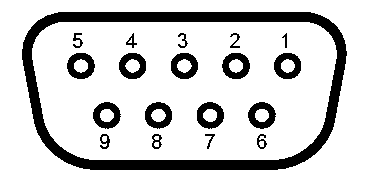
\includegraphics[width=5cm]{grafiken/Numbered_DE9_female_Diagram.pdf}
\end{minipage}
\hspace{1cm}
\begin{minipage}[h]{5cm}
\begin{tabular}{|c|c|}
\hline 
\textbf{Pin} & \textbf{Description} \\ \hline 
1 & Bridge B output 1 \\ \hline 
2 & Bridge B output 2 \\ \hline 
3 & Bridge A output 2 \\ \hline 
4 & Bridge A output 1 \\ \hline 
5 & Ground \\ \hline 
6 & \unit[+5]{V} \\ \hline 
7 & Reference/Limit Switch 1 \\ \hline 
8 & Reference/Limit Switch 2 \\ \hline 
9 & Reference/Limit Switch 3 \\ \hline 
\end{tabular}
\end{minipage}
\end{center}
\caption[Pinout of the Motor Connector.]{Pinout of the Motor Connector.}
\label{pin_out}
\end{figure}










\newpage

\clearpage


\newpage
\printindex

\end{document}















